\section{Theory}

We briefly summarize the theoretical underpinnings of the NPRR algorithm to provide further understanding and underscore our motivation for studying this algorithm. A detailed survey of this algorithm (and its more general version, known as Generic Join) can be found in \cite{ngo2014skew} and \cite{ngo2012worst}.

Traditional mult-way join queries (join queries that involve $n$ relations, where $n > 2$) are evaluated by using a cost-based estimation model to determine the best pair-wise join plan \cite{shapiro1986join}. This, however, is provably suboptimal in the worst-case; to see this, consider the triangle query:
\begin{align*}
Q = R(A, B) \bowtie S(B, C) \bowtie T(A, C)
\end{align*}

Without loss of generality, suppose this query was executed using the pair-wise join plan $(R \bowtie S) \bowtie T$. If $|R| = |S| = N$, then the intermediate relation $P = R \bowtie S$ will have cardinality $|P| = O(N^2)$ in the worst case. However, the size of the intermediate relation does not provide a lower bound for the size of the final output. If $|T| = N$ as well, then the subsequent join $P \bowtie T$ may, in the best case, generate a final output of $N^2$ tuples. However, in the worst case, $P \bowtie T$ may only generate $O(N)$ tuples, or even no tuples at all.

Thus, we can always construct a family of instances that will provably have $\Omega(N^2)$ runtime; figure \ref{fig:triangle} illustrates this in more detail. Moreover, we know by the \texttt{AGM} bound that the upper bound for the output for the triangle query is $O(N^{3/2})$ \cite{atserias2008size}. Ngo et al. demonstrate that there is a family of algorithms that does achieve this bound. We discuss the intuition for this algorithm strictly for the case of triangle queries below; a more general and thorough treatment of the algorithm (as well as detailed pseudocode) can be found in \cite{ngo2012worst} and \cite{ngo2014skew}.

\begin{figure}[h]
\label{fig:triangle}
\begin{center}
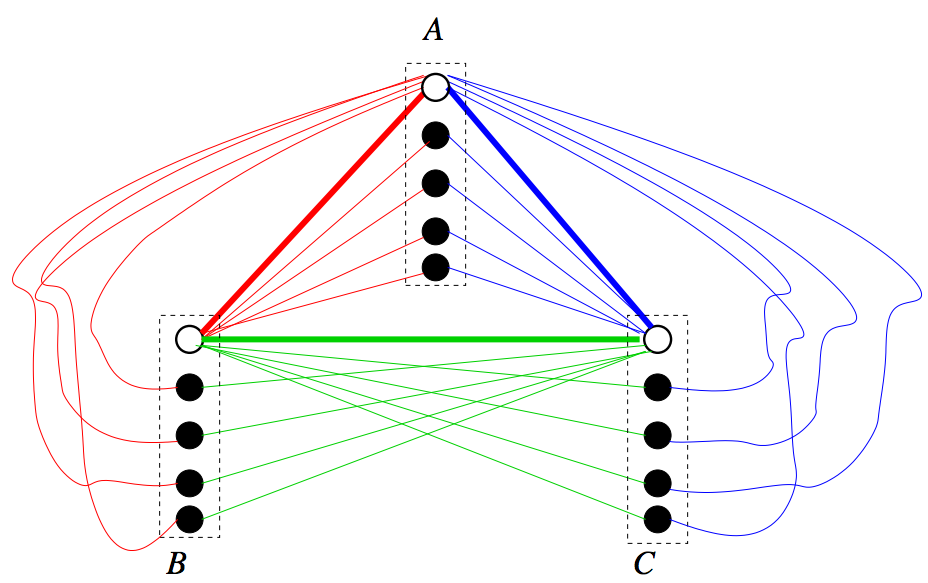
\includegraphics[scale=0.2]{triangle.png}
\end{center}
\caption{A counter-example which demonstrates why pair-wise plans for the triangle query are suboptimal. See \cite{ngo2014skew} for a thorough explanation.}
\end{figure}

First, rather than fix an order of relations to join, we instead fix some order of \emph{attributes}. Doing so enables us to ``look ahead'' and ensure that we don't unnecessarily materialize an intermediate relation that could prove to be wasteful later on in the computation. Without loss of generality, let our order $U = (A, B, C)$. We first compute candidates for attribute $A$, which we denote as $C_A$. To do this, we examine each relation with $A$ in its attribute set, and then compute the following: $C_A = \pi_A (R) \cap \pi_A (T)$. We can now guarantee that, for every possible triangle $(a_i, b_j, c_k)$ in the final output, $a_i \in C_A$ will always hold true. In other words, $C_A$ gives us the list of candidate values for attribute $A$ that may participate in the final output.

Next, we compute candidates for attribute $B$, which is next in our order $U$. We use the same approach as before, but we now incorporate our $C_A$ candidate values. For each $a_i \in C_A$, we evaluate $C_{AB} = \{a_i\} \times \big(\pi_B (\sigma_{A = a_i} R) \cap \pi_B (T)\big)$. Just as before, we maintain the invariant that every tuple $(a_i, b_j) \in C_{AB}$ is a candidate tuple for the final output.

Lastly, for attribute $C$, we iterate through each candidate $(a_i, b_j) \in C_{AB}$, and evaluate $C_{ABC} = \{a_i, b_j\} \times \big(\pi_C (\sigma_{B = b_j} S) \cap \pi_C (\sigma_{A = a_i} T)\big)$. The candidate set $C_{ABC}$ now equals our final output.

\begin{figure}[h]
\label{fig:walkthrough}
  \begin{minipage}[b]{0.55\linewidth}
  \centering
  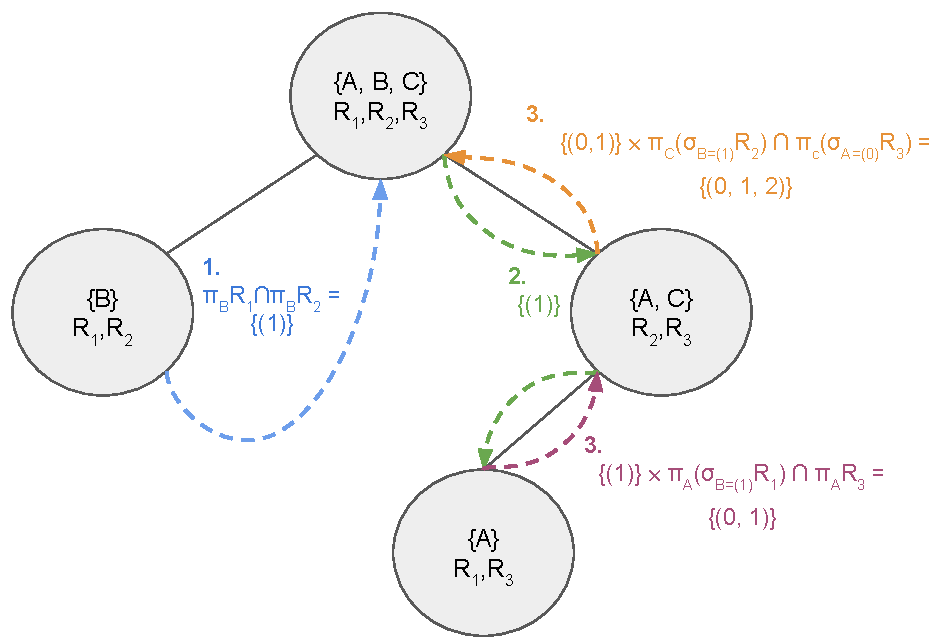
\includegraphics[scale=0.55]{walkthrough.pdf}
  \end{minipage}
  \begin{minipage}[b]{0.45\linewidth}
  \centering
  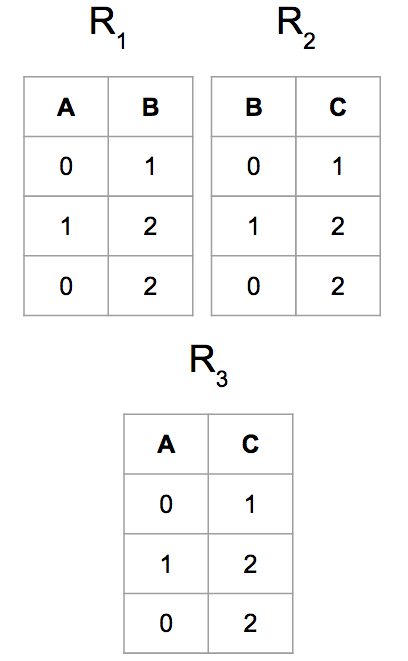
\includegraphics[scale=0.22]{table_walkthrough.png}
  \end{minipage}
\caption{A walkthrough of the NPRR algorithm on the triangle query. Here the attribute order $U = (B,A, C)$.}
\end{figure}